\chapter{ManagedIrbis. Быстрый старт}

У попа была собака. Он её любил. Она съела кусок мяса. Он её убил. В землю закопал. Надпись написал. У попа была собака. Он её любил. Она съела кусок мяса. Он её убил. В землю закопал. Надпись написал.

У попа была собака. Он её любил. Она съела кусок мяса. Он её убил. В землю закопал. Надпись написал. У попа была собака. Он её любил. Она съела кусок мяса. Он её убил. В землю закопал. Надпись написал. У попа была собака. Он её любил. Она съела кусок мяса. Он её убил. В землю закопал. Надпись написал.

У попа была собака. Он её любил. Она съела кусок мяса. Он её убил. В землю закопал. Надпись написал.

У попа была собака. Он её любил. Она съела кусок мяса. Он её убил. В землю закопал. Надпись написал.

У попа была собака. Он её любил. Она съела кусок мяса. Он её убил. В землю закопал. Надпись написал. У попа была собака. Он её любил. Она съела кусок мяса. Он её убил. В землю закопал. Надпись написал.

\begin{figure}[h]
	\centering
	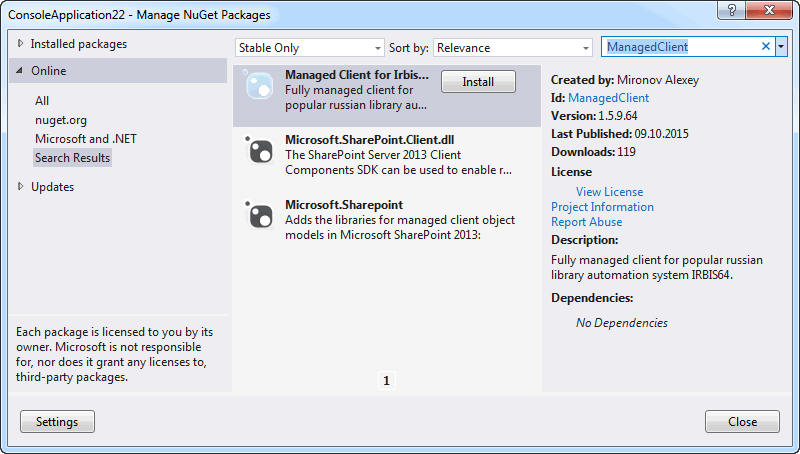
\includegraphics[width=0.7\textwidth]{nuget}
	\caption{Подключение библиотеки через NuGet}
\end{figure}


\begin{lstlisting}
using System;
using System.Linq;

using ManagedIrbis;

class Program
{
  private static void Main()
  {
    try
    {
      using (IrbisConnection connection = new IrbisConnection())
      {
        connection.ParseConnectionString
          (
            "host=127.0.0.1;port=6666;user=1;password=1;"
          );
        connection.Connect();

        int[] foundRecords = connection.Search
          (
            "\"A={0}$\"",
            "А"
          );

        int recordsToShow = Math.Min(foundRecords.Length, 10);

        for (int i = 0; i < recordsToShow; i++)
        {
          int thisMfn = foundRecords[i];

          MarcRecord record = connection.ReadRecord(thisMfn);

          string mainTitle = record
            .Fields
            .GetField("200")
            .GetSubField('a')
            .GetSubFieldText()
            .FirstOrDefault();

          Console.WriteLine
            (
              "MFN={0}, Main title={1}",
              thisMfn,
              mainTitle
            );

          Console.WriteLine
            (
              "BRIEF: {0}",
              client.FormatRecord("@brief", record)
            );

          MarcRecord newRecord = new MarcRecord();
          newRecord.AddField
            (
              "700",
              'a',
              "Управляемый клиент ИРБИС64"
            )
            .AddField
            (
              "200",
              'a', 
              string.Format ("Новая Запись от {0}", DateTime.Now),
              'f',
              "Управляемый клиент"
            );

          connection.WriteRecord
            (
              newRecord, 
              false, 
              true
            );

          Console.WriteLine(new string('-', 60));
        }
      }
    }
    catch (Exception ex)
    {
      Console.WriteLine(ex);
    }
  }
}\end{lstlisting}
